\section{Model Fitting using MCMC}
We fit each model using a sequential scan Metropolis-Hastings algorithm where we visit each component of the parameters in turn, and for each component, $j$ propose $X_{j} \sim q_{j}(\cdot \mid X_{1}^{(t)}, \ldots, X_{j-1}^{(t)},$ $X_{j}^{(t-1)}, \ldots, X_{d}^{(t-1)})$.\footnotemark~For each run, we simulate a Markov chain of length $10,000$ and select a sub-sample for every $100$ step. We summarize below the diagnostic plots of the MCMC outputs from model 2. The Markov chain demonstrates good convergence properties. From the trace plots of the parameters $\lambda^{(t)}, \beta^{(t)}$, the log-likelihood and the log-prior (Figure~ \ref{fig:4a}), it is observed that the chain is stationary from the beginning of the simulation, suggesting that no burn-in period is required and we can keep the entire chain. In addition, no obvious trends in the trace plots are observed, suggesting good explorations of the parameter space of the target posterior density. \footnotetext{This proposal is chosen such that the prior and the proposal cancels when evaluating the acceptance probability, and we are only left with the likelihood ratio.}

\begin{figure}[ht!]
\centering
\begin{subfigure}[b]{0.45\textwidth} \centering
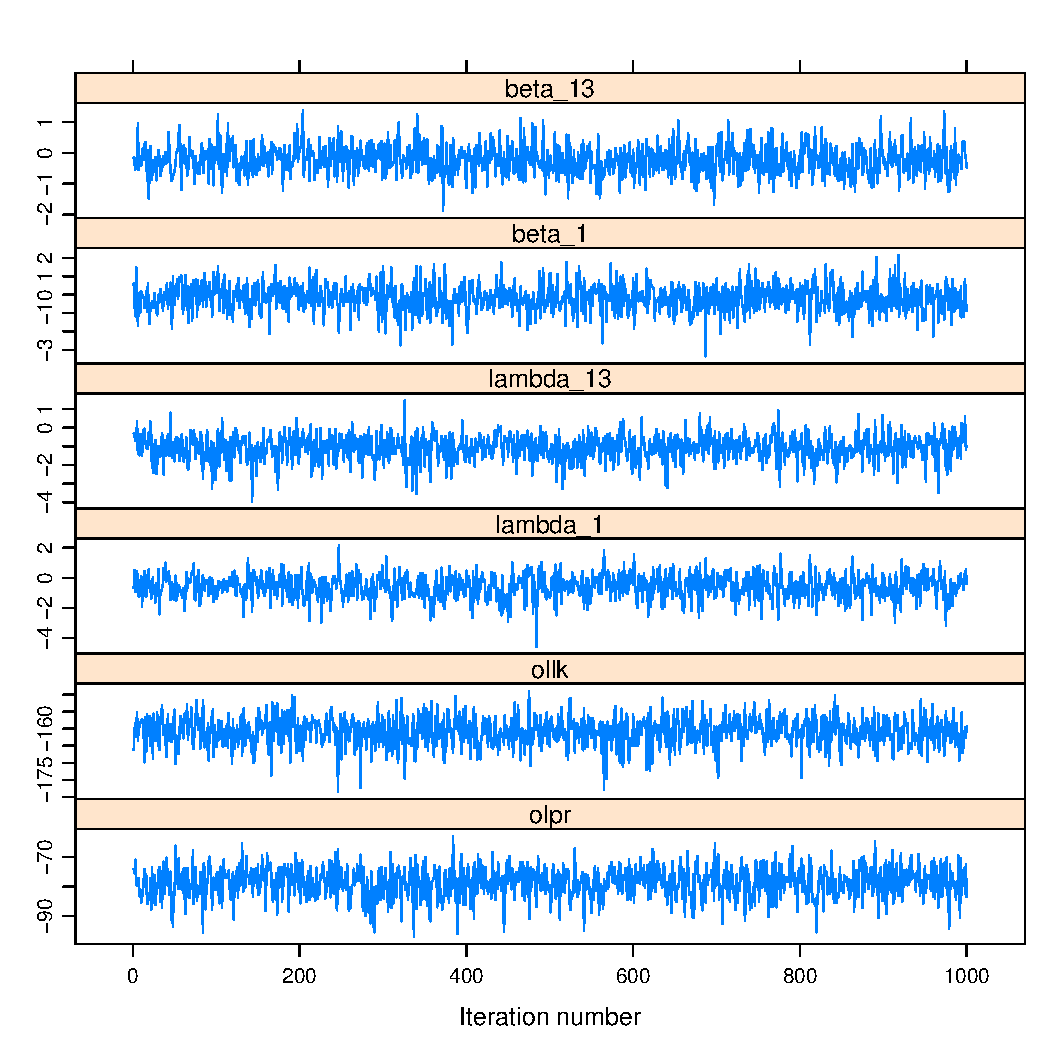
\includegraphics[width=0.95\linewidth]{xyplot}
\caption{Trace plots of the MCMC outputs}
\label{fig:4a}
\end{subfigure}
\begin{subfigure}[b]{0.45\textwidth} \centering
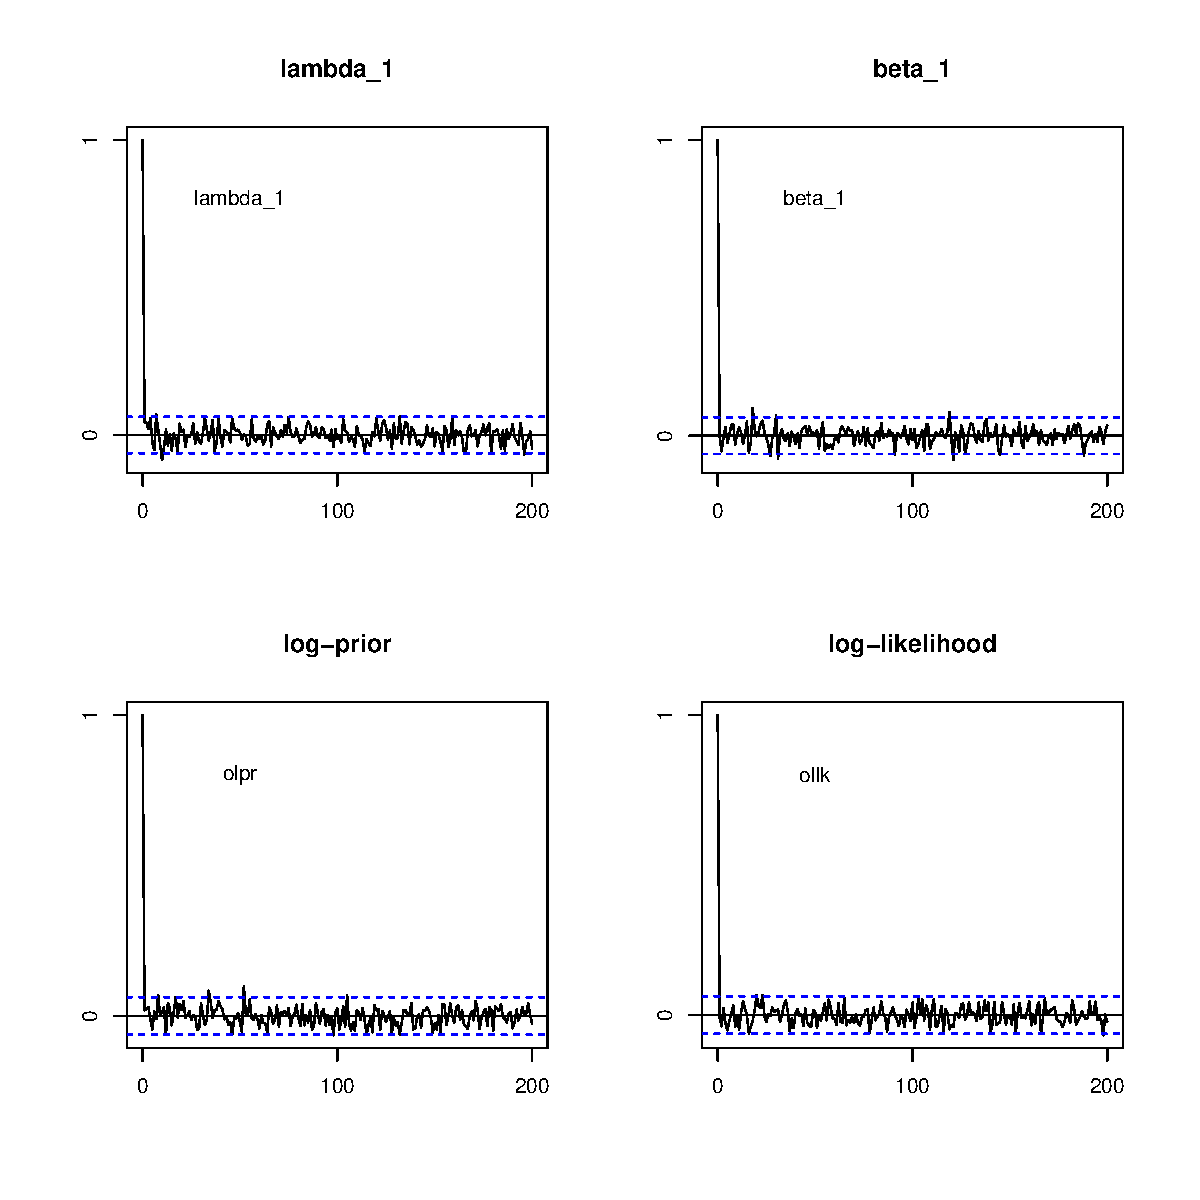
\includegraphics[width=0.95\linewidth]{acf}
\caption{ACFs of the MCMC outputs}
\label{fig:4b}
\end{subfigure} \hspace{1em}
\caption{MCMC output diagnostics: (Left) Trace plots of the variables and key functions. (Right) ACFs of the trace plots.
The trace plots are stationary from the beginning, and the ACFs fall off to zero rapidly. Both plots suggest good exploration of the parameter space and convergence properties of the MCMC.} \label{fig:4}
\end{figure}

Figure~\ref{fig:4b} summarizes the auto-correlation for the MCMC output sequences. The auto-correlation falls off to zero quickly, and the effective sample size of all parameters is close to the number of sub-samples $1000$ (the number of iterations divided by the step size). We perform multiple runs from different start states and check those marginal distributions agree in Figure~\ref{fig:5}, which again confirms the good convergence of the chain to the target distribution.
\begin{figure}[ht!]
\centering
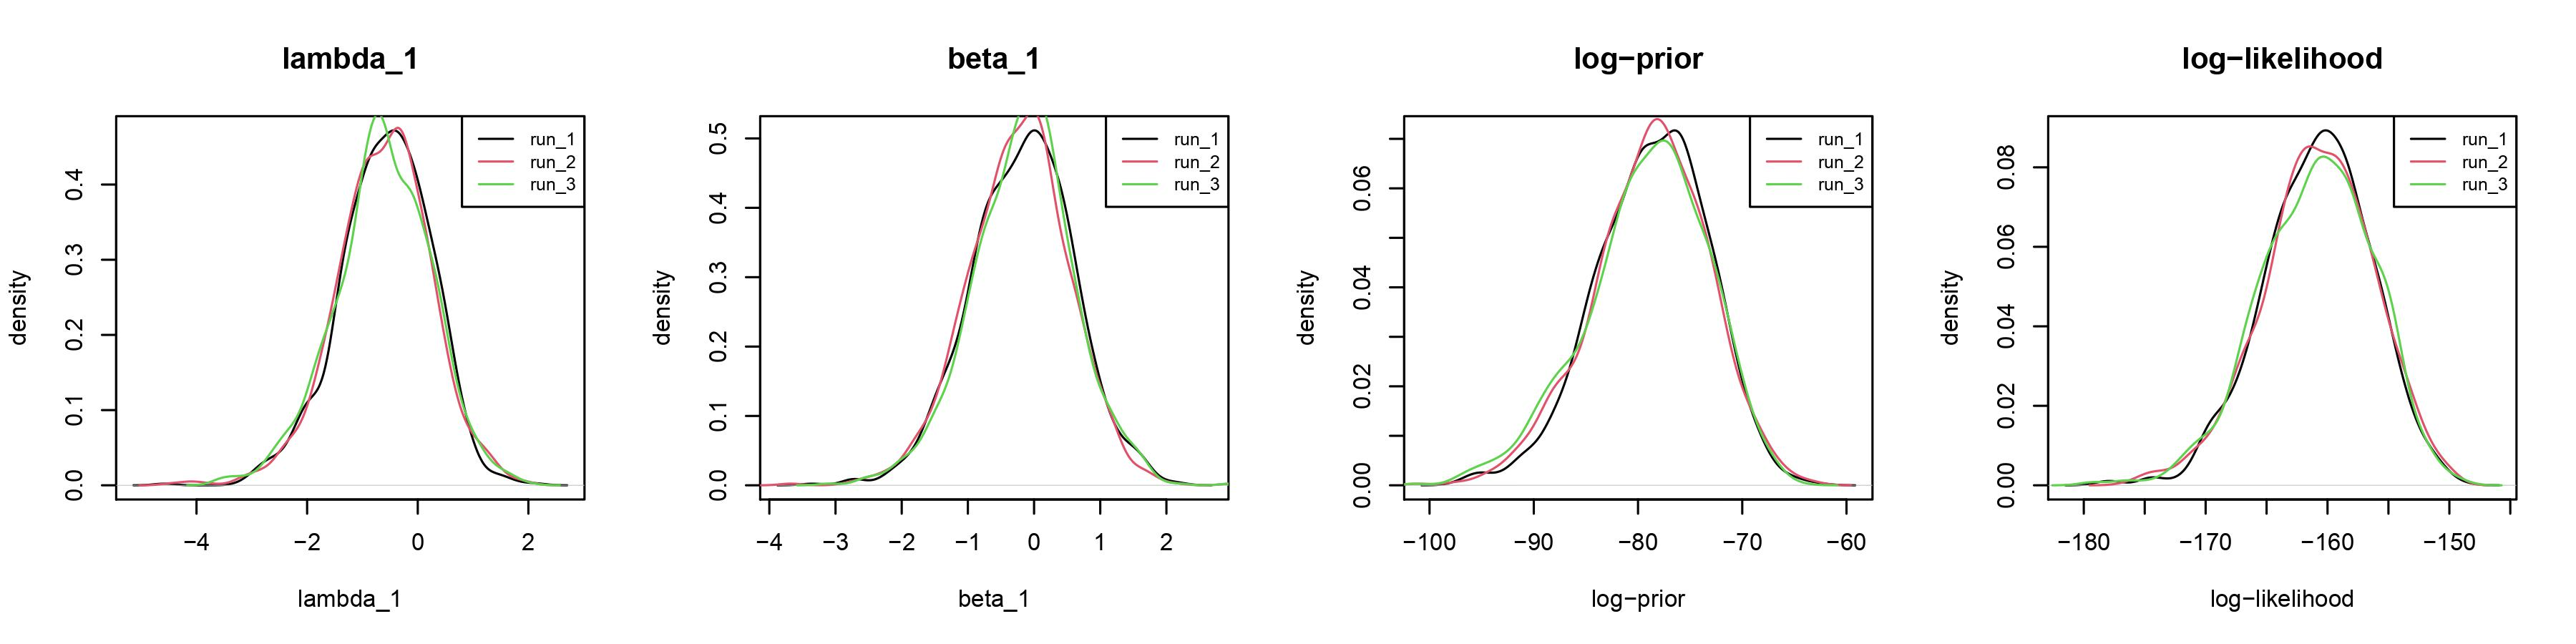
\includegraphics[width=1.0\linewidth]{runs}
\caption{Density plots of the variables and key functions in three runs with different start states}
\label{fig:5}
\end{figure}
